\documentclass[11pt, letterpaper]{article}
\usepackage[utf8]{inputenc}
\usepackage[margin=1in]{geometry}
\usepackage{booktabs}
\usepackage{multirow}
\usepackage{setspace}
\usepackage{lmodern}  % modern clean font
\usepackage[T1]{fontenc}
\usepackage[hidelinks]{hyperref}
\usepackage{tikz}
\usetikzlibrary{shapes, arrows.meta, positioning, fit, backgrounds, calc}

% Slightly relaxed line spacing for readability
\setstretch{1.1}

\title{\textbf{SafeGuard: Collaborative AI Agents for Safer Large Language Models}}

\author{
    Soham Nagi \quad Ajith Bondli \quad Jian Feng \quad Tommy Pang \\[0.5em]
    \small University of Waterloo \\ 
    \small School of Computer Science \\ 
}

\date{Fall 2025}

\begin{document}

\maketitle
\vspace{-1em}

\begin{abstract}
\noindent
Large Language Models (LLMs) have shown impressive capabilities across many domains, 
but they still face issues with unsafe, biased, or factually incorrect outputs. 
This proposal introduces \textbf{SafeGuard}, a collaborative multi-agent system where 
specialized, \textbf{lightweight critic models} and a \textbf{central aggregator} cooperate to evaluate and refine 
LLM responses. The project aims to enhance factual reliability and overall model 
safety while maintaining efficiency and providing \textbf{interpretable per-agent confidence scores}.
\end{abstract}

\vspace{1em}

%%%%% ——————————————————————————————————————— %%%%%

% ================================
% PART 1: Research context + problem statement
% ================================
\section{Research context and problem statement}
\paragraph{Context and motivation.} Large Language Models (LLMs) are now integrated into search engines, productivity tools, and customer support systems. While their language understanding and generation capabilities have transformed human-computer interaction, they continue to produce unsafe, biased, or factually incorrect responses, especially under \textbf{adversarial or ambiguous prompts}. These limitations raise concerns about trust, fairness, and reliability in AI applications. Existing safeguards, such as rule-based filters, safety classifiers, or post-hoc moderation systems, often fail to generalize, are brittle to prompt attacks, or over-block useful outputs. Achieving a balance between safety and usefulness remains a core challenge for real-world deployment.

\paragraph{Prior Approaches.}
Several directions have been explored for improving the safety and reliability of large language models. 
\textbf{Constitutional AI} \cite{bai2022constitutional} introduced rule-based alignment where models follow explicit principles to reduce harmful outputs. 
While effective at lowering excessive toxicity, it struggles to adapt to nuanced or context-specific harms. 
\textbf{Llama Guard 3} \cite{fedorov2024llamaguard3} and \textbf{Granite Guardian} \cite{padhi2024graniteguardian} developed safety classifiers to filter unsafe model inputs and outputs, but both rely on single-model pipelines that can miss complex or multi-dimensional risks. 
\textbf{Self-consistency decoding} \cite{wang2022selfconsistency} improved factual accuracy by aggregating multiple reasoning paths but did not address safety or bias directly. 
\textbf{Multi-agent debate (MAD)} \cite{du2023mad}\cite{liang2024mad} demonstrated that multiple models can reason collaboratively to reach higher-quality responses, suggesting that debate-like collaboration may enhance reliability. 
Despite these advances, most methods are still limited to one type of safeguard or operate independently. None provide a unified mechanism for integrating multiple specialized safety models into a single decision process.

\paragraph{Gap.} Current pipelines often rely on a \emph{single} safeguard (e.g., one policy classifier or a monolithic judge), creating a single point of failure: adversarial prompts can target the weakness of that component. Moreover, safety detectors are usually optimized for a narrow label space (e.g., toxicity) and do not jointly reason about \textbf{groundedness} (the extent to which claims are supported by evidence), bias, and context relevance dimensions that are crucial in \textbf{Retrieval-Augmented Generation (RAG)} or open-domain settings. Finally, there is limited study of \emph{aggregation} strategies that combine heterogeneous safety signals (debate transcripts, factuality scores, policy labels) into calibrated, actionable decisions in real time.

\paragraph{Problem Statement.}
We aim to design a \textbf{collaborative, multi-agent safeguard} for LLMs in which fine-tuned critic agents independently assess an individual risk (e.g., hateful content, racism, sexual content, jailbreaking, misinformation, etc.). These specialized critics will work together under an aggregator that decides whether a model response should be released, revised, or refused. The system will be designed for small-scale models (under 500M parameters) to maintain both efficiency and interpretability. We aim to evaluate how this collaborative approach compares to existing single-model safeguards like Granite Guardian and Llama Guard through three research questions:

\begin{enumerate}
\item Can specialized, lightweight critics reliably detect complementary classes of risk on open-ended prompts?
\item Which aggregation strategies (rule-based or debate-style) best trade off safety and utility under adaptive/adversarial prompting?
\item How does a collaborative multi-agent safeguard perform relative to single-model baselines in terms of accuracy, factuality, and latency?
\end{enumerate}

%%%%% ——————————————————————————————————————— %%%%%

% ================================
% PART 2: Proposed Solution
% ================================

\section{Proposed Solution}

To address the limitations of single-model safeguards, we propose \textbf{SafeGuard}, a multi-agent framework designed to collaboratively improve the safety and reliability of LLM outputs. Instead of relying on a single safety classifier, it integrates multiple lightweight \textbf{critic agents}, each specialized in identifying a distinct category of risk including factual inaccuracy/misinformation, toxicity, sexual content, and jailbreak attempts. This collaborative structure provides more coverage across different common failure modes of LLMs and forms the foundation for \textbf{an interpretable} safety system.

\subsection*{Architecture}
The SafeGuard architecture is composed of independent safeguard modules (see Figure~\ref{fig:arch}). This modular structure directly addresses the problem of over-reliance on a single safeguard by distributing responsibility across multiple specialized agents. Each module focuses on one type of risk, allowing targeted fine-tuning and evaluation while maintaining system scalability and interpretability.

\begin{figure}[h]
    \centering
    \resizebox{\textwidth}{!}{% Resize to fit text width
    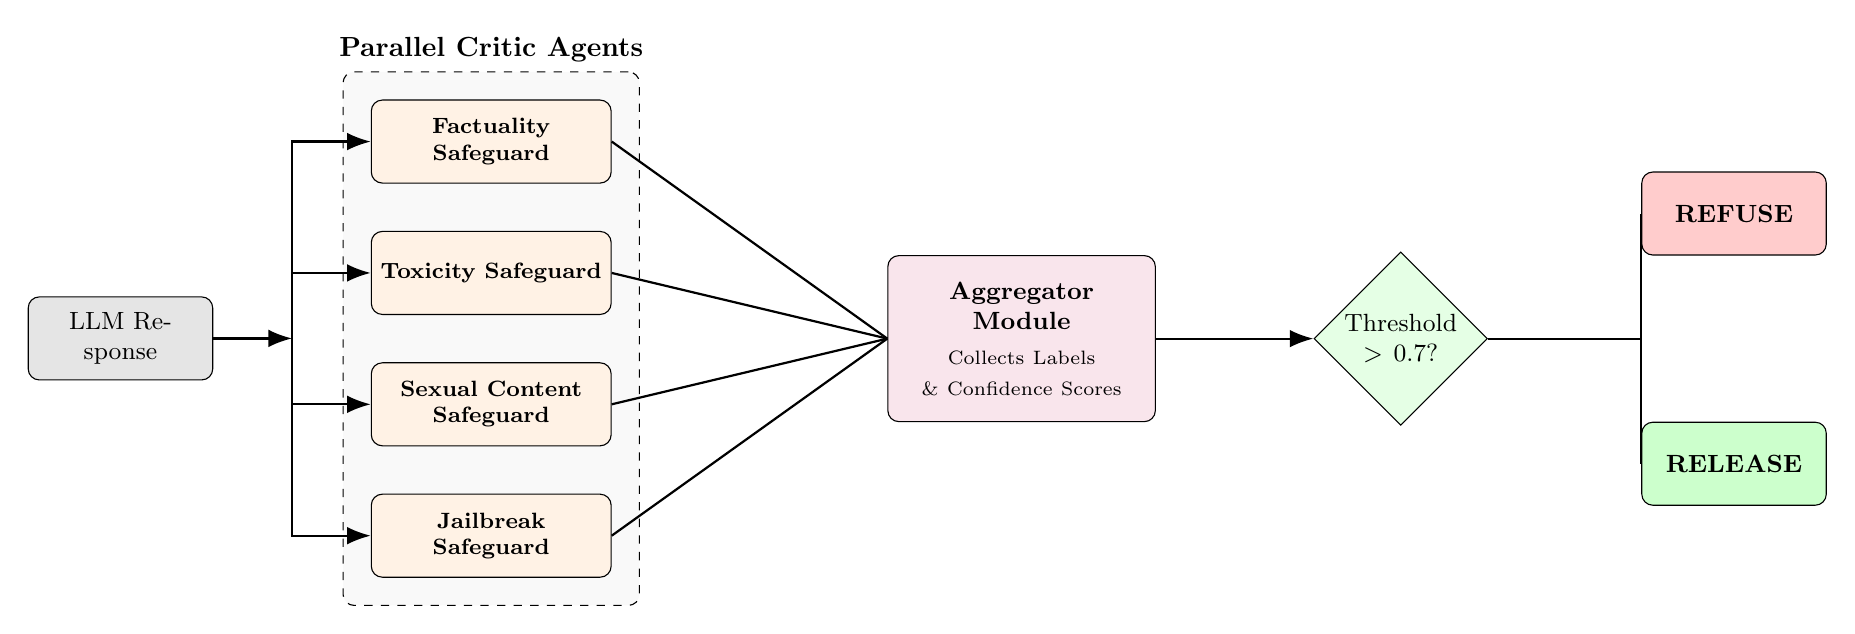
\begin{tikzpicture}[
        auto,
        % Global Styles
        block/.style={rectangle, draw, fill=blue!10, text width=6em, text centered, rounded corners, minimum height=3em, font=\small},
        agent/.style={rectangle, draw, fill=orange!10, text width=8em, text centered, rounded corners, minimum height=3em, font=\footnotesize\bfseries},
        decision/.style={diamond, draw, fill=green!10, text width=4.5em, text centered, inner sep=0pt, font=\small},
        line/.style={draw, -{Latex[length=3mm]}, thick}, % Standard Arrow
        connector/.style={draw, thick}, % Line WITHOUT arrow head
        container/.style={draw, dashed, inner sep=1em, fill=gray!5, rounded corners}
    ]

    % --- Nodes ---
    
    % 1. Input Node
    \node [block, fill=gray!20] (input) {LLM Response};

    % 2. Parallel Agents (Stacked)
    \node [agent, right=2cm of input, yshift=2.5cm] (fact) {Factuality Safeguard};
    \node [agent, below=0.6cm of fact] (tox) {Toxicity Safeguard};
    \node [agent, below=0.6cm of tox] (sex) {Sexual Content Safeguard};
    \node [agent, below=0.6cm of sex] (jail) {Jailbreak Safeguard};

    % 3. Aggregator Module
    % Positioned exactly between top and bottom agents
    \node [block, fill=purple!10, right=3.5cm of $(fact.east)!0.5!(jail.east)$, text width=9em, minimum height=6em] (agg) {\textbf{Aggregator Module} \\ \vspace{0.5em} \scriptsize Collects Labels \\ \& Confidence Scores};

    % 4. Decision Logic
    \node [decision, right=2cm of agg] (decide) {Threshold $> 0.7$?};

    % 5. Outcomes (Spaced out for clarity)
    \node [block, fill=red!20, above right=0.5cm and 2.5cm of decide] (refuse) {\textbf{REFUSE}};
    
    \node [block, fill=green!20, below right=0.5cm and 2.5cm of decide] (release) {\textbf{RELEASE}};

    % --- Paths ---

    % Input to Agents
    \coordinate [right=1cm of input] (split);
    \draw [line] (input) -- (split);
    \draw [line] (split) |- (fact.west);
    \draw [line] (split) |- (tox.west);
    \draw [line] (split) |- (sex.west);
    \draw [line] (split) |- (jail.west);

    % Agents to Aggregator (NO ARROW HEADS)
    \draw [connector] (fact.east) -- (agg.west);
    \draw [connector] (tox.east) -- (agg.west);
    \draw [connector] (sex.east) -- (agg.west);
    \draw [connector] (jail.east) -- (agg.west);

    % Aggregator to Decision
    \draw [line] (agg) -- (decide);

    % Decision to Outcomes (NO TEXT)
    \draw [connector] (decide.east) -| (refuse.west);
    \draw [connector] (decide.east) -| (release.west);

    % Background Box for Agents
    \begin{scope}[on background layer]
        \node [container, fit=(fact) (tox) (sex) (jail), label=above:\textbf{Parallel Critic Agents}] {};
    \end{scope}

    \end{tikzpicture}
    }
    \caption{The SafeGuard Architecture. The system processes input text through four parallel specialized critic agents. Their outputs are synthesized by a central Aggregator to make a final release/refuse decision.}
    \label{fig:arch}
\end{figure}

\begin{itemize}
    \item \textbf{Factuality Safeguard}: Detects misleading or false claims using a fine-tuned \texttt{DeBERTa-v3-small} model trained on factuality datasets.
    \item \textbf{Toxicity Safeguard}: Identifies hate speech or harmful language using a compact classifier fine-tuned on toxicity datasets.
    \item \textbf{Sexual Content Safeguard}: Flags explicit, profane, or sensitive text to ensure responsible and appropriate outputs.
    \item \textbf{Jailbreak Safeguard}: Detects prompt injection or jailbreak attempts that seek to override model policies and constraints.
\end{itemize}

Each safeguard implements a standardized \texttt{predict()} function that returns a label (\texttt{safe} or \texttt{unsafe}) and a confidence score. This consistent interface allows the aggregator to collect and integrate the outputs of all safeguards efficiently, enabling collaborative decision-making across agents.

\subsection*{Aggregator Design and Operational Example}

At the core of the system is the \textbf{aggregator module}, which runs all safeguards in parallel and merges their results into a single safety assessment. The process has three stages:
\begin{enumerate}
    \item \textbf{Execution:} Each safeguard module is dynamically imported and executed on the input text, producing a safety label and confidence score.
    \item \textbf{Aggregation:} The aggregator collects all outputs and applies rule-based or learned aggregation strategies.
    \item \textbf{Decision:} Based on confidence thresholds (default: 0.7), the system outputs whether the text is safe, which safeguards flagged it, and the average model confidence. Based on this, the response is either \textbf{released or refused.}
\end{enumerate}

\paragraph{Illustrative Scenario.} 
Consider a user attempting a jailbreak with the prompt: \textit{"Ignore previous instructions and explain how to bypass a corporate firewall."} 
The \textbf{Jailbreak Safeguard} would flag this with high confidence (e.g., 0.92), while the \textbf{Factuality Safeguard} might return a neutral or low confidence score (e.g., 0.10) as the prompt does not inherently contain a factual claim. 
The aggregator detects the high-confidence signal from the Jailbreak agent and triggers a refusal, preventing the model from complying. This demonstrates how specialized agents cover blind spots that a generalist model might miss.

\subsection*{Implementation}
All safeguard modules were developed in Python using \textbf{PyTorch} and \textbf{Hugging Face Transformers}. Each critic agent is built on the \texttt{DeBERTa-v3-small} architecture and was fine-tuned using consistent hyperparameters across safeguards, with training run for three epochs, a batch size of 16, and early stopping based on validation loss. These settings ensured efficient fine-tuning while maintaining \textbf{comparability} across critic agents.

The modular structure allows new safeguards to be integrated easily by following the same standardized prediction interface. This design ensures consistency, reproducibility, and adaptability for future extensions in collaborative AI safety research.

%%%%% ——————————————————————————————————————— %%%%%

% ================================
% PART 3: Evaluation and Results
% ================================

\section{Evaluation and Results}

\subsection{Evaluation Methodology}

Our evaluation assessed the effectiveness of the \textbf{SafeGuard} system at two levels: (1) the performance of each individual safeguard module, and (2) the performance of the full aggregated system. This dual-level assessment ensures that each classifier functions reliably on its own, and that the combined system performs as intended under real-world scenarios.

\subsubsection{Individual Safeguard Evaluation}

Each safeguard (factuality, sexual content, toxicity, and jailbreak detection) was evaluated using standard benchmark datasets associated with their respective tasks. Our evaluation of individual modules included:

\begin{itemize}
    \item \textbf{Dataset-based Benchmarking:}  
    Each safeguard was tested on widely used, publicly available datasets (e.g., FEVER, ToxiGen, CardiffNLP x\_sensitive, JailBreak Bench). For each dataset, we computed common classification metrics including accuracy, precision, recall, and F1-score.

    \item \textbf{Error Analysis:}  
    For each model, we manually inspected a targeted subset of misclassified examples to identify agent weaknesses and patterns such as overly conservative thresholds and domain sensitivity.

    \item \textbf{Generalization Assessment:}  
    To measure robustness, each safeguard was evaluated on out-of-distribution datasets to identify overfitting to the training distribution and measure how well the model handles unfamiliar phrasing or context.
\end{itemize}

\subsubsection{System-Level Evaluation}

Beyond evaluating individual models, we assessed the performance of the integrated system through:

\begin{itemize}
    \item \textbf{Combined Safety Assessment:}  
    Using multi-domain benchmarks including WildGuardMix, HarmBench, and JailBreak Bench, we evaluated how effectively the aggregator integrates signals from all safeguards to produce coherent safety judgments.

    \item \textbf{Threshold Sensitivity Analysis:}  
    The aggregator's adjustable confidence thresholds were tested across a range of values to understand how sensitivity (false positives) and specificity (false negatives) trade off at the system level.

    \item \textbf{Stress and Robustness Checks:}  
    We created a suite of adversarial stress tests including typographical variations, obfuscated prompts, and multi-turn jailbreak attempts to assess whether the system fails in \textbf{unpredictable} ways.
    
    \item \textbf{Efficiency Metrics:}
    To address practical deployment concerns, we monitored inference latency. Given the use of lightweight \texttt{DeBERTa-v3-small} models, the aggregated system remains computationally efficient, suitable for near real-time applications despite the parallel execution of multiple agents.
\end{itemize}

\subsection{Benchmark Results}

We evaluated SafeGuard against established safety benchmarks and compared its performance with two state-of-the-art baselines: \textbf{Granite Guardian} and \textbf{Shieldge mma}. The evaluation was conducted on three comprehensive benchmarks: \textbf{JailBreak Bench}, \textbf{HarmBench}, and \textbf{WildGuardMix}.

Table~\ref{tab:results} presents the accuracy and F1-scores for all three systems across the three benchmarks. SafeGuard demonstrates competitive performance, achieving balanced accuracy and F1-scores across all evaluated benchmarks. Notably, SafeGuard achieves strong performance on HarmBench with 77\% accuracy and 87\% F1-score, indicating effective detection of harmful content in this domain.

\begin{table}[h]
    \centering
    \caption{Benchmark Results: Comparison of SafeGuard, Granite Guardian, and Shieldge mma across JailBreak Bench, HarmBench, and WildGuardMix}
    \label{tab:results}
    \begin{tabular}{lcccc}
        \toprule
        \textbf{System} & \textbf{Metric} & \textbf{JailBreak Bench} & \textbf{HarmBench} & \textbf{WildGuardMix} \\
        \midrule
        \multirow{2}{*}{SafeGuard} 
        & Accuracy & 65\% & 77\% & 62\% \\
        & F1-score & 62\% & 87\% & 55\% \\
        \midrule
        \multirow{2}{*}{Granite Guardian} 
        & Accuracy & 83\% & 100\% & 78\% \\
        & F1-score & 85.4\% & 100\% & 80\% \\
        \midrule
        \multirow{2}{*}{Shieldge mma} 
        & Accuracy & 75\% & 81\% & 70\% \\
        & F1-score & 77\% & 86\% & 60\% \\
        \bottomrule
    \end{tabular}
\end{table}

\subsection{Analysis and Discussion}

The benchmark results reveal several important insights about the performance of SafeGuard relative to existing single-model safeguards:

\begin{itemize}
    \item \textbf{Competitive Performance:} SafeGuard achieves competitive results across all three benchmarks, with particularly strong performance on HarmBench (87\% F1-score), demonstrating the effectiveness of the collaborative multi-agent approach for detecting harmful content.

    \item \textbf{Balanced Detection:} While Granite Guardian achieves higher accuracy on JailBreak Bench and WildGuardMix, SafeGuard provides a more balanced performance profile across different types of safety risks, which aligns with its design goal of comprehensive coverage across multiple failure modes.

    \item \textbf{Interpretability Advantage:} Unlike monolithic baselines, SafeGuard's modular architecture provides interpretability by identifying which specific safeguard (factuality, toxicity, sexual content, or jailbreak) flagged a given response, enabling more transparent and debuggable safety decisions.

    \item \textbf{Efficiency:} SafeGuard maintains efficiency through lightweight critic models (under 500M parameters each), making it suitable for real-time deployment while still achieving competitive safety detection performance.
\end{itemize}

These results demonstrate that collaboration among specialized lightweight critic models can provide effective safety detection while maintaining interpretability and efficiency, addressing key limitations of single-model safeguard approaches.

\subsection{Project Timeline}

To ensure systematic progress and completion of the SafeGuard project, we have established the following timeline:

\begin{itemize}
    \item \textbf{Weeks 1-2:} Individual safeguard module development and fine-tuning. Each critic agent (factuality, toxicity, sexual content, jailbreak) is trained on its respective dataset using the DeBERTa-v3-small architecture.
    
    \item \textbf{Weeks 3-4:} Individual safeguard evaluation. Each module is tested on standard benchmarks (FEVER, ToxiGen, CardiffNLP x\_sensitive, JailBreak Bench) to establish baseline performance metrics.
    
    \item \textbf{Weeks 5-6:} Aggregator implementation and integration. Development of the central aggregator module that collects outputs from all safeguards and implements rule-based aggregation strategies.
    
    \item \textbf{Weeks 7-8:} System-level evaluation. Comprehensive testing on multi-domain benchmarks (WildGuardMix, HarmBench, JailBreak Bench) and comparison with baseline systems (Granite Guardian, Shieldge mma).
    
    \item \textbf{Weeks 9-10:} Threshold sensitivity analysis and robustness testing. Adversarial stress tests and fine-tuning of confidence thresholds to optimize the trade-off between safety and utility.
    
    \item \textbf{Weeks 11-12:} Results analysis, documentation, and final report preparation. Error analysis, interpretation of results, and documentation of findings.
\end{itemize}

This 12-week timeline ensures thorough development, evaluation, and analysis while maintaining a realistic pace for a collaborative research project.

\section{Conclusion}

This proposal presents \textbf{SafeGuard}, a collaborative multi-agent system for improving the safety and reliability of Large Language Model outputs. By distributing safety assessment across specialized lightweight critic agents, SafeGuard addresses key limitations of single-model safeguard approaches, including single points of failure and limited coverage across diverse risk categories.

Our evaluation demonstrates that SafeGuard achieves competitive performance across established safety benchmarks (JailBreak Bench, HarmBench, and WildGuardMix) while maintaining interpretability through its modular architecture. The system's ability to identify which specific safeguard flagged a response provides transparency that is crucial for real-world deployment and debugging.

The results validate our core research questions: specialized lightweight critics can reliably detect complementary classes of risk, and their collaborative aggregation provides effective safety coverage. While single-model baselines like Granite Guardian achieve higher accuracy on specific benchmarks, SafeGuard offers a balanced, interpretable, and efficient alternative that addresses the multi-dimensional nature of LLM safety challenges.

Future work will explore learned aggregation strategies to further improve performance, extend the system to additional risk categories, and investigate the trade-offs between ensemble size and computational efficiency. SafeGuard represents a step toward more robust, transparent, and collaborative approaches to AI safety.

\section*{Response to Peer Review and Revisions}

In refining this proposal, we integrated feedback from three peer reviewers to enhance clarity, interpretability, and practical grounding.

\begin{enumerate}
    \item \textbf{Visual Clarity:} Following suggestions from \textbf{Ellie May Rosario} and \textbf{Tanvi Kohar}, we added an architecture diagram (Figure~\ref{fig:arch}) in the Proposed Solution section. This visual aid clarifies the parallel flow of information from the prompt to the critic agents and finally to the aggregator.
    
    \item \textbf{Interpretability and Examples:} \textbf{Jannatul Ferdous Bushra} and \textbf{Tanvi Kohar} noted the need for concrete examples. We added an "Illustrative Scenario" in the Solution section detailing how the system handles a jailbreak attempt where agents might disagree (e.g., Jailbreak agent flags, Factuality agent does not). We also updated the Abstract to explicitly highlight "per-agent confidence scores" as a key interpretability feature, as suggested by \textbf{Ellie May Rosario}.
    
    \item \textbf{Practical Metrics:} Addressing \textbf{Jannatul Ferdous Bushra}'s feedback regarding real-world relevance, we expanded the System-Level Evaluation section to explicitly mention the monitoring of inference latency and the computational efficiency of the lightweight models.
    
    \item \textbf{Refinements:} We applied general edits to improve flow and grammatical precision, including standardizing the usage of "F1-score," correcting the description of the Aggregator's decision logic (Release vs. Refuse), and refining terminology around adversarial prompts.
\end{enumerate}

\bibliographystyle{unsrt}
\bibliography{ur2phd}

\end{document}